\documentclass[6pt]{article}

%Landscape orientation
\usepackage[margin=1cm,landscape]{geometry}
% Collumn rulers
\setlength{\columnseprule}{0.3pt}
\def\columnseprulecolor{\color{grey}}

%Userpackages
\usepackage[utf8]{inputenc}
\usepackage[T1]{fontenc}
\usepackage{multicol} % For three collumns
\usepackage{mcode} %Matlab code color and font
\usepackage{amsmath} %For \text
\usepackage{graphicx} %For figures
\graphicspath{ {images/} }
\usepackage{commath} % For \abs{}
\usepackage{amsthm} %for theorem
\usepackage{enumitem}
\usepackage{hyperref} % For \url and \hyperref
\usepackage{resizegather} % Scale gather environ to \linewidth

% Custom commands
\newcommand*\diff{\mathop{}\!\mathrm{d}}
\newcommand*\Diff[1]{\mathop{}\!\mathrm{d^#1}} % For \diff{}{}
\newcommand*\conj[1]{\overline{#1}} % Seperate conjugate command
\newcommand*\magn[1]{||#1||} % Seperate magnitude command
\theoremstyle{definition}
\newtheorem*{theorem*}{Theorem}
\newtheorem*{theorem}{Theorem}
\newtheorem*{definition}{Definition} %for definition
\newtheorem*{definition*}{Definition} %for unnumbered definition

% Custom settings
\pagestyle{empty} %Turn off header and footer

\makeatletter % Redefine section commands to use less space
\renewcommand{\section}{\@startsection{section}{1}{0mm}%
                                {-1ex plus -.5ex minus -.2ex}%
                                {0.5ex plus .2ex}%x
                                {\normalfont\large\bfseries}}
\renewcommand{\subsection}{\@startsection{subsection}{2}{0mm}%
                                {-1explus -.5ex minus -.2ex}%
                                {0.5ex plus .2ex}%
                                {\normalfont\normalsize\bfseries}}
\renewcommand{\subsubsection}{\@startsection{subsubsection}{3}{0mm}%
                                {-1ex plus -.5ex minus -.2ex}%
                                {1ex plus .2ex}%
                                {\normalfont\small\bfseries}}
\makeatother

% Don't print section numbers
\setcounter{secnumdepth}{0}

\setlength{\parindent}{0pt}
\setlength{\parskip}{0pt plus 0.5ex}

%Turn off display of date in title
\date{}

% Less space above and below equations
\AtBeginDocument{%
  \setlength\abovedisplayskip{7pt}
  \setlength\belowdisplayskip{7pt}}

\title{TMA4320 Cheat Sheet}

\begin{document}

% Three collumns
\begin{multicols*}{3}

\maketitle
v1.0.2 (TeX source @ \href{https://github.com/JakobGM/Numerical-Analysis-Cheat-Sheet}{GitHub.com/JakobGM/})
\section{Solving equations}
\begin{definition}
The function $f(x)$ has a \textbf{root} at $x = r$ if $f(r) = 0$.
\end{definition}

\subsubsection{The Bisection Method}
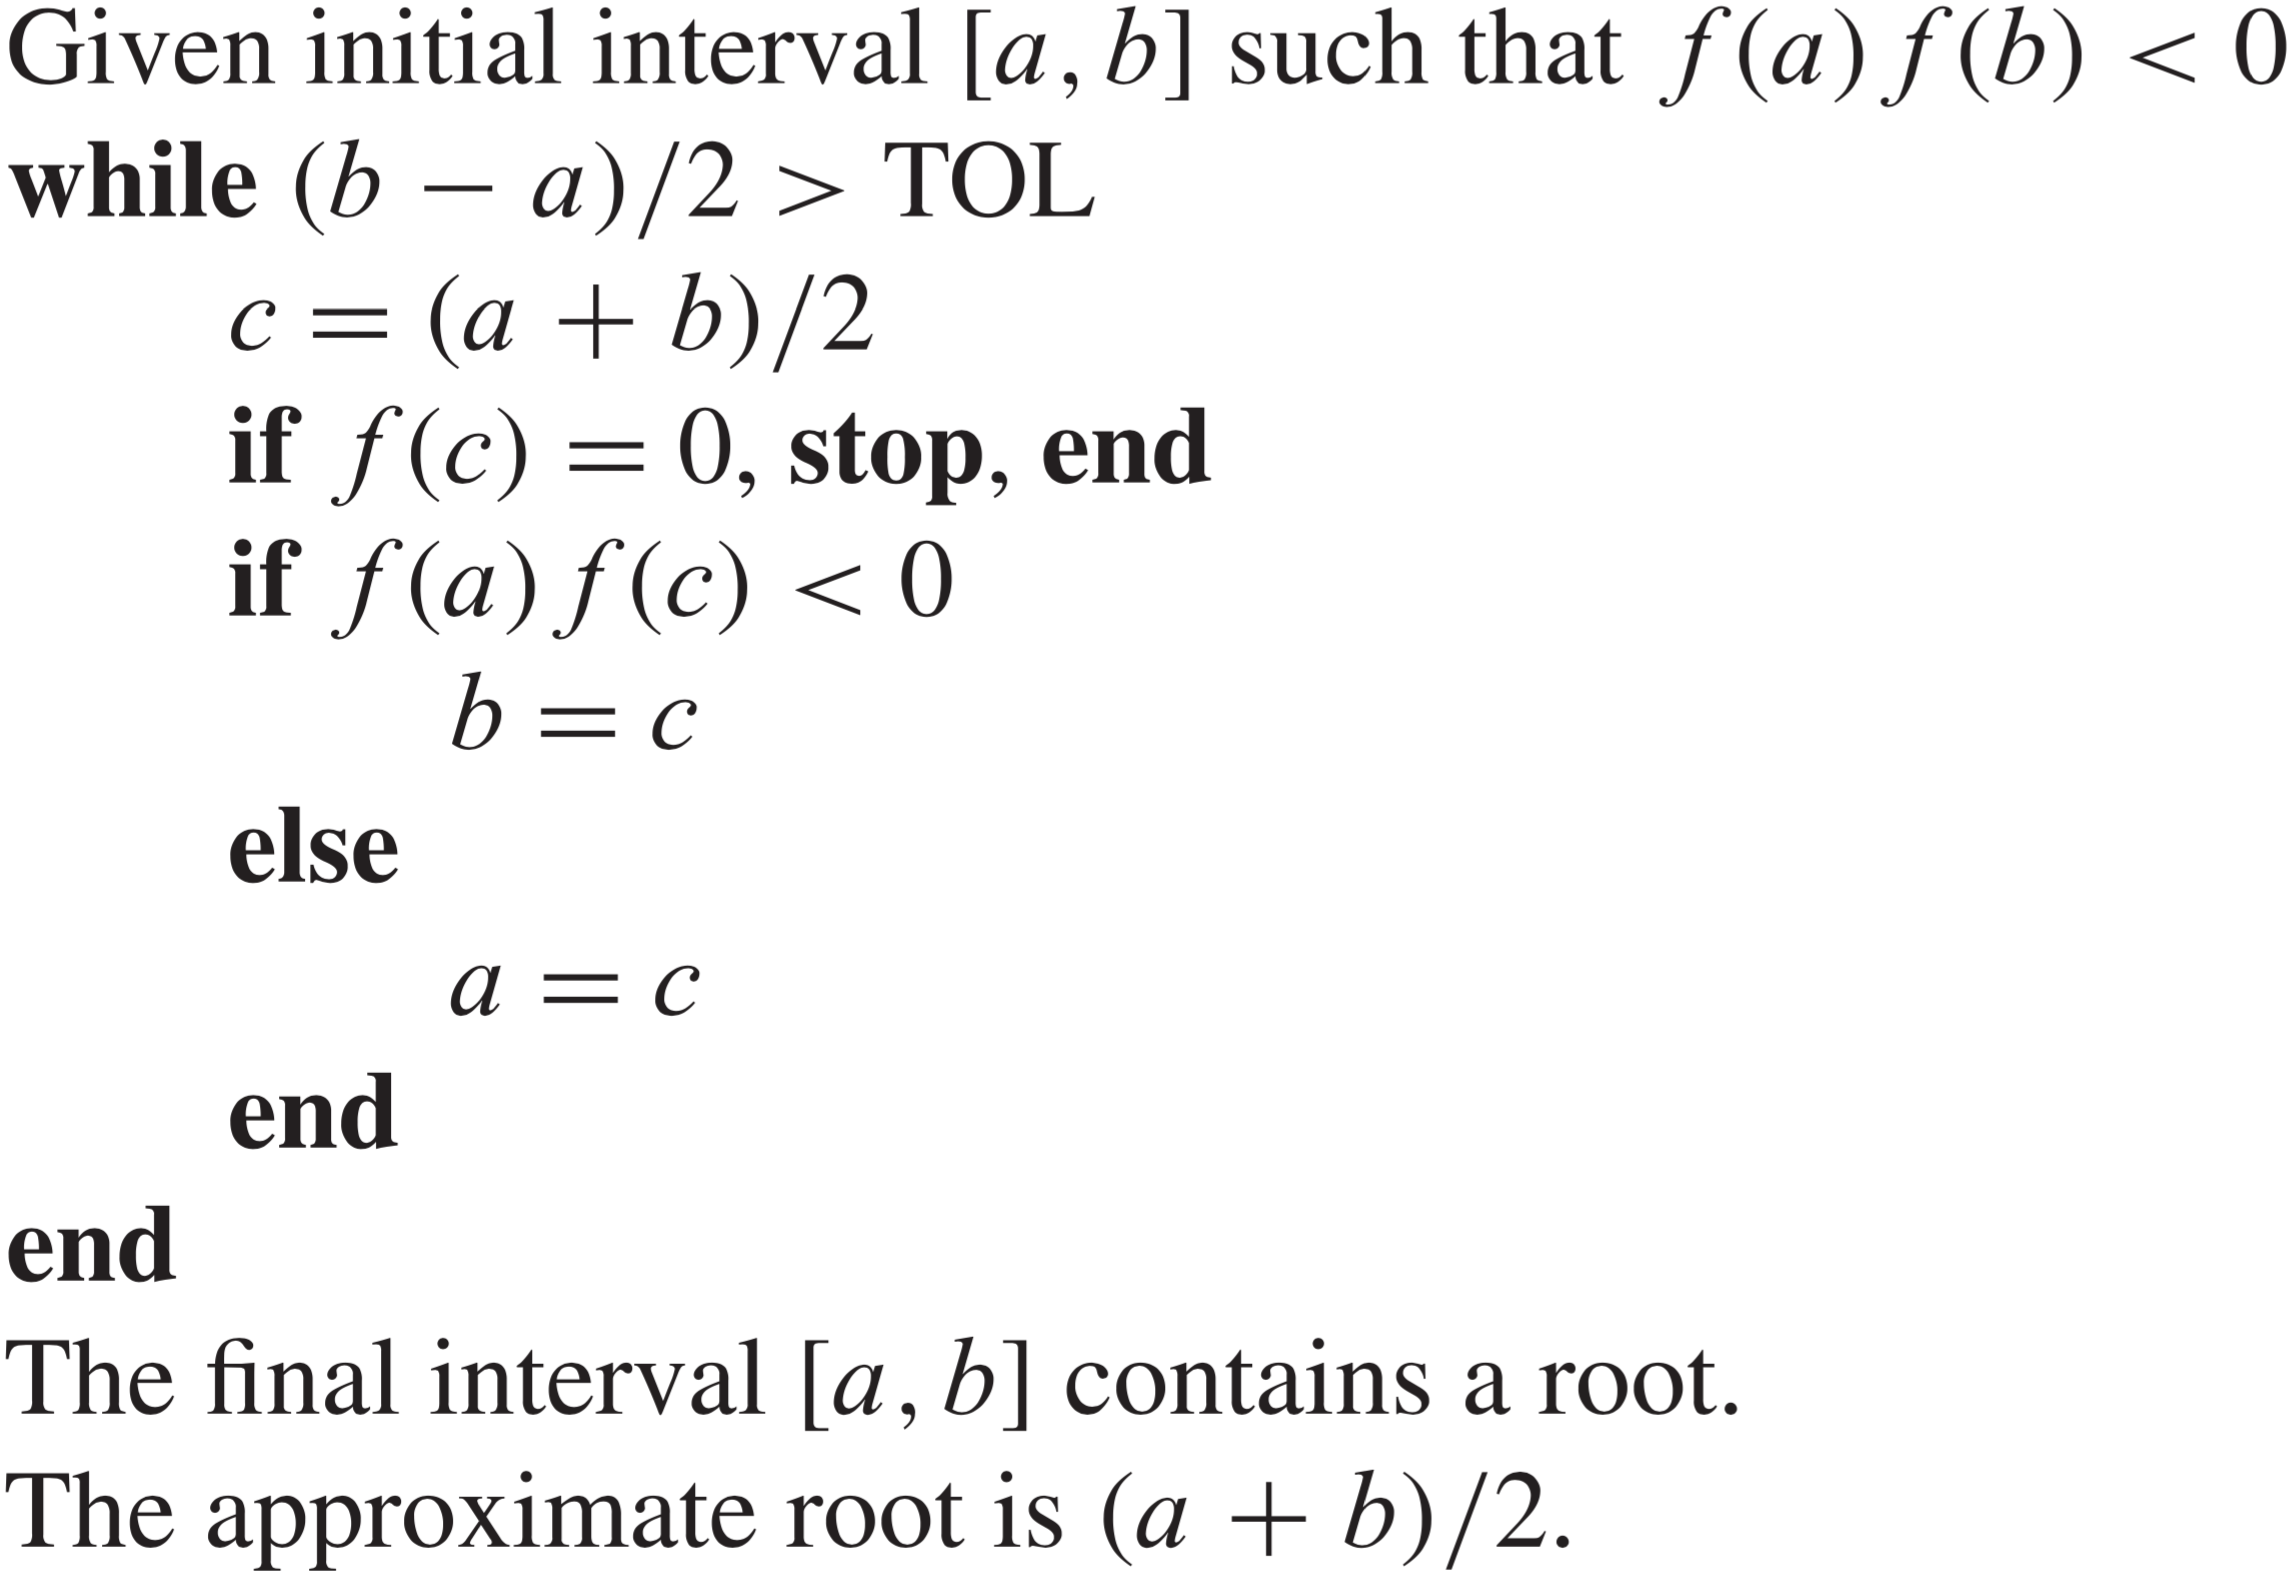
\includegraphics[scale=0.17]{images/bisection_method.png}

% Written pseudocode in MatLab pseudosyntax, men used the book instead (see above)
% \begin{lstlisting}
% %Given initial interval [a,b] such that f(a)f(b)<0
% while (b-a)/2 < TOL
%     c = (a + b)/2;
    
%     if f(c) == 0
%         %End
%     if f(a)*f(c) < 0
%         b = c;
%     else
%         a = c;
% end
% % The final interval [a,b] contains a root
% % The approximate root is (a + b)/2
% \end{lstlisting}

\begin{gather*}
\text{Solution error} = |x_c - r| < \frac{b-a}{2^{n+1}} \\
\text{Function evaluations} = n + 2
\end{gather*}
\subsubsection{Fixed point iteration}
\begin{gather*}
x_0 = \text{initial guess} \\
x_{i+1} = g(x_i) \textbf{ for } i = 0,1,2,... \\
\end{gather*}

\begin{lstlisting}
%Function handle g
% Starting guess x0
% Number of iteration steps k
function xc = fpi(g, x0, k)
x(1) = x0;

for i = 1:k
    x(i+1) = g(x(i));
end

xc = x(k+1);
\end{lstlisting}

\begin{theorem*}
Assume that $g$ is continously differentiable, that $g(r) = r$, and that $S = |f'(r)| < 1$. The Fixed-Point Iteration converges linearly with the rate $S$ to the fixed point $r$ for initial guesses sufficiently close to $r$.
\end{theorem*}

\subsubsection{Newton's method} 
\begin{gather*}
x_0 = \text{initial guess} \\
x_{i+1} = x_i - \frac{f(x_i)}{f'(x_i)} \text{ \textbf{for} i = 0,1,2,...}
\end{gather*}

\begin{theorem*}
Let $f$ be twice continuously differentiable and $f(r) = 0$. If $f'(r) \neq 0$, then Newton's method is locally and quadratically convergent to $r$. The error $e_i$ at step $i$ satisfies
$$
\lim_{i \to \infty} \frac{e_{i+1}}{e_{i}^2} = M,
$$
where
$$
M = \frac{f''(r)}{2f'(r)}.
$$
\end{theorem*}

\begin{theorem*}
Assume that the $(m+1)$-times continously differentiable function $f$ on $[a,b]$ has a multiplicity $m$ at root $r$. Then Newton's Method is locally convergent to $r$, and the error $e_i$ at step $i$ satisfies
$$
\lim_{i \to \infty} \frac{e_{i+1}}{e_{i}} = S
$$
%where $S = {m-1}{m}$
\end{theorem*}

\begin{theorem*}
If $f$ is $(m+1)$-times continuously differentiable on $[a,b]$, which contains a root $r$ of multiplicity $m > 1$, the the \textbf{Modified Newton's Method}
$$
x_{i+1} = x_i - \frac{m f(x_i)}{f'(x_i)}
$$
converges locally and quadratically to $r$.
\end{theorem*}
\hfill 
\section{Interpolation}
\subsubsection{Lagrange interpolation}
The \textit{unique} degree $n-1$ polynomial that interpolates the $n$ datapoints $(x_1, y_1), ..., (x_n, y_n)$ is given by
$$
P_{n-1}(x) = y_1L_1(x) + ... + y_nL_n(x)
$$
where $L_k$ is given by
$$
L_k(x) = \frac{(x-x_1)...(x-x_{k-1})(x-x_{k+1})...(x-x_n)}{(x_k-x_1)...(x_k - x_{k-1})(x_k - x_{k+1})...(x_k-x_n)}
$$

\subsubsection{Netwon's divided differences}
\begin{definition}
Denote by $f[x_1...x_n]$ the coefficients of the $x^{n-1}$ term in the (unique) polynomial that interpolates $(x_1, f(x_1)), ..., (x_n,f(x_n))$.
\end{definition}

\begin{center}
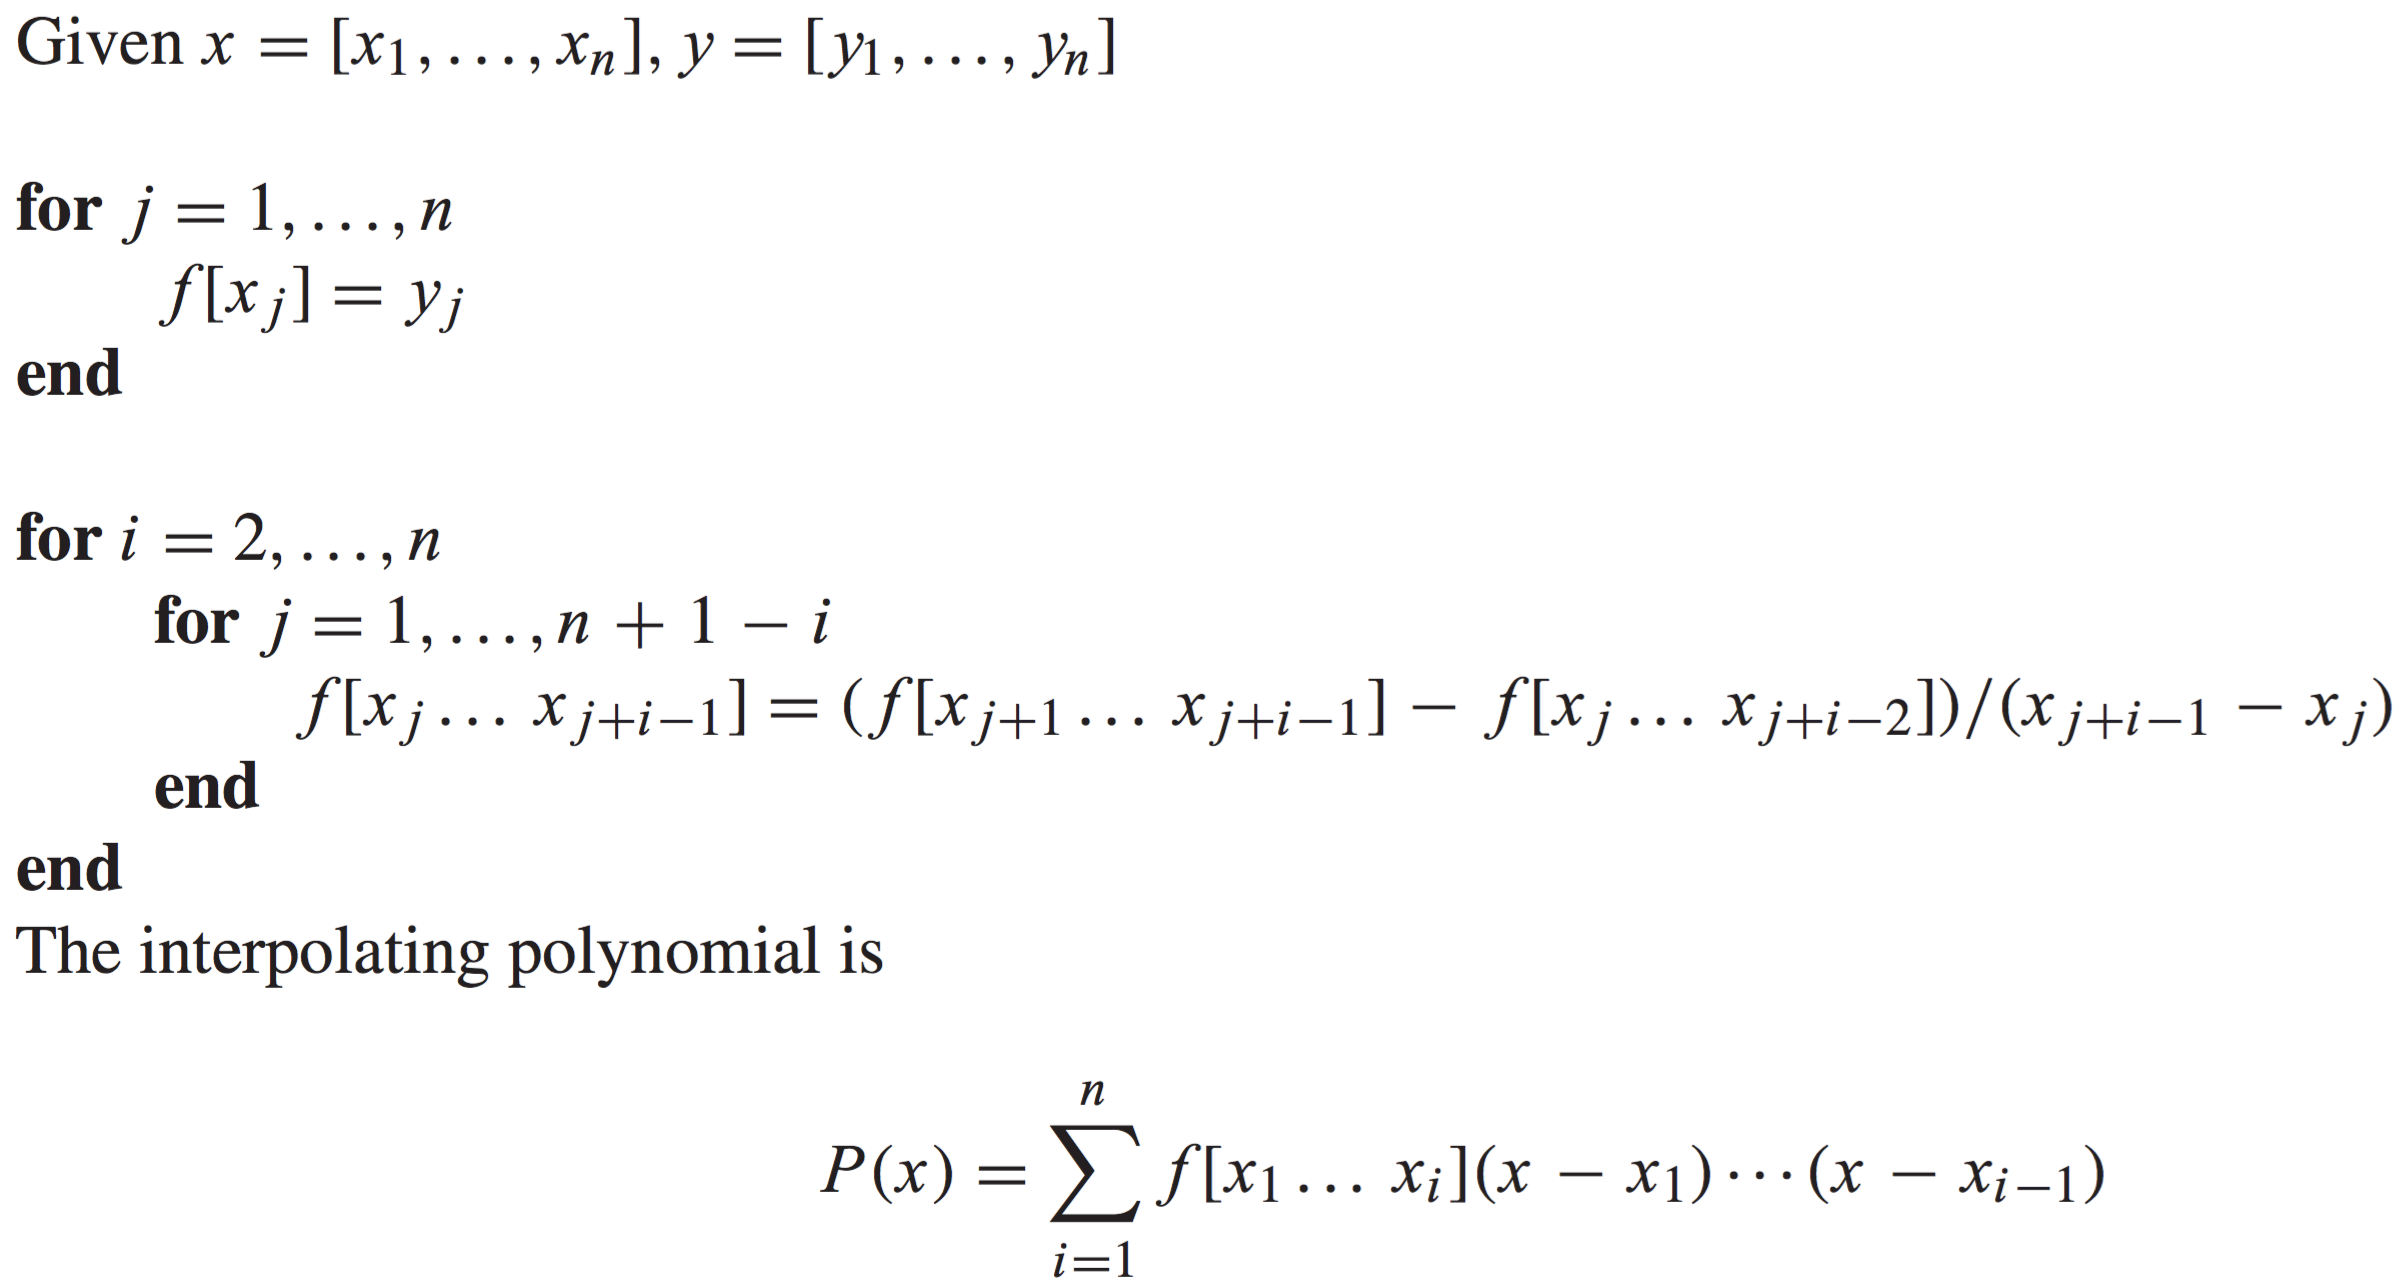
\includegraphics[scale=0.22]{newtondd_algorithm.png}
\end{center}

When writing by hand, use a table like this to calculate the differences
\begin{center}
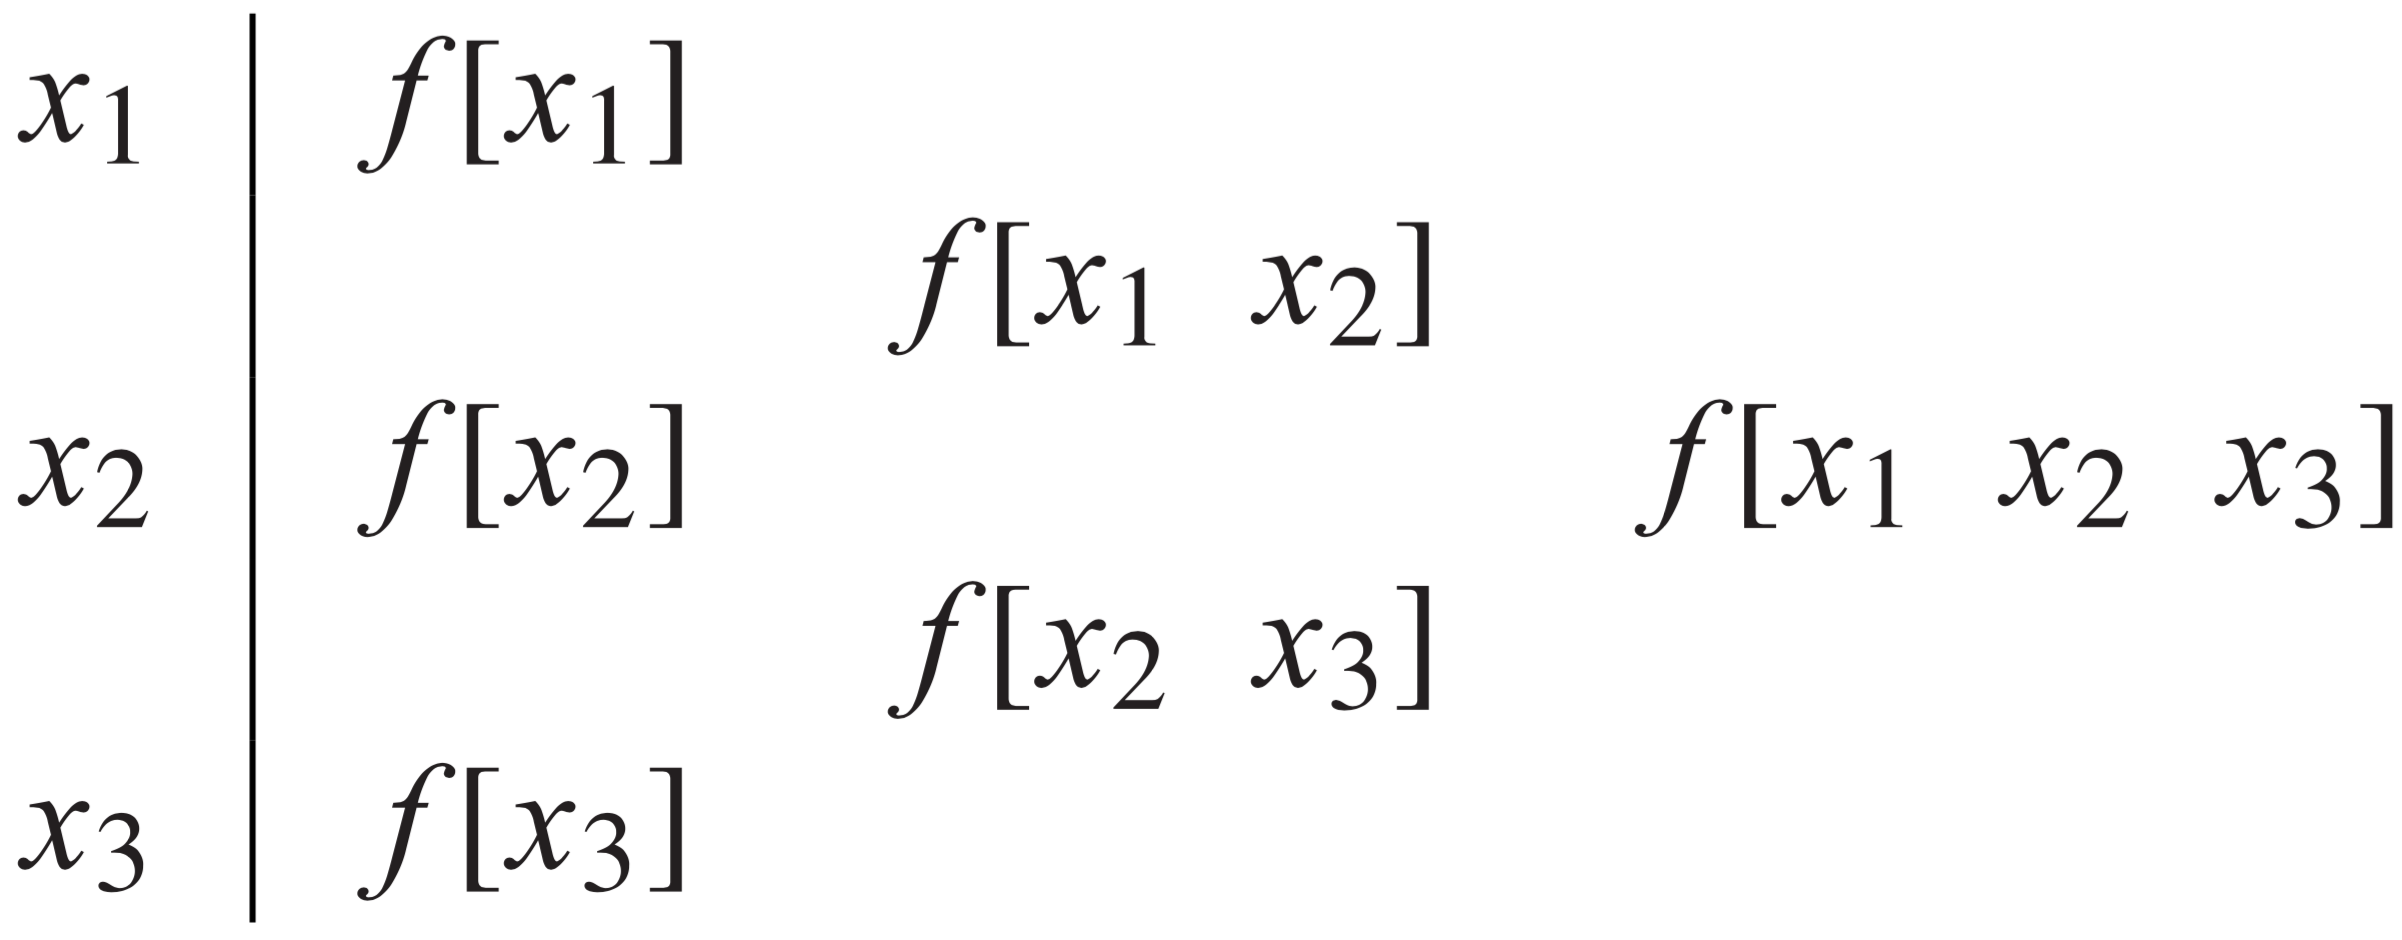
\includegraphics[scale=0.1]{newtondd.png}
\end{center}

\subsubsection{Interpolation error}
%You should have an idea about where the interpolation error estimate comes from, but do not memorize the exact form.

\begin{theorem}
$P(x)$, the degree $n-1$ or less interpolation of $n$ points, has an intepolation error of
$$
f(x) - P(x) = \frac{(x-x_1)(x-x_2)...(x-x_n)}{n!}f^{(n)}(c)
$$
where $c \in [\text{min}(x_1,...,x_n), \text{max}(x_1,...,x_n)]$. Find the upper bound.
\end{theorem}

\begin{theorem}
Assume that $P(x)$ is the (degree $n-1$ or less) interpolating polynomial fitting the $n$ points $(x_1,y_1),...,(x_n,y_n)$. The interpolation error is
$$
f(x)-P(x) = \frac{(x-x_1)(x-x_2)...(x-x_n)}{n!}f^{(n)}(c),
$$
where $c \in [\text{max}(x_1,...,x_n), \text{min}(x_1,...,x_n)]$.
\end{theorem}

\subsubsection{Runge's phenomenon}
Runge's phenomenon is the consequence of the magnitude of the derivatives of the interpolation function grows quickly when n increases. This causes a "wiggle" effect at the ends of the interval and is solved by redistributing the interpolation nodes. Speaking of which...

\subsubsection{Chebyshev Interpolation Nodes}
\begin{theorem}
On the interval $[a,b]$,
$$
x_i = \frac{b+a}{2} + \frac{b-a}{2}\cos{\frac{(2i-1)\pi}{2n}}
$$
for $i = 1, ..., n$. The inequality
$$
|(x-x_1)...(x-x_n)| \leq \frac{(\frac{b-a}{2})^n}{2^{n-1}}
$$
holds on $[a,b]$
\end{theorem}
\section{Numerical quadratures}
Methods for integrating $f(x)$ on the interval $[a,b]$, using $m$ points. The used variable $c$ is always contained in this interval.
%Formulas for the most basic Newton-Cotes quadratures, at least trapezoid and mid-point. 

\subsection{Composite Trapezoid Rule}
$$
\int_{a}^{b} f(x) \diff{x} = \frac{h}{2}(y_0+y_m + 2\sum_{i=1}^{m-1}y_i) - \frac{(b-a)h^2}{12}f''(c),
$$
where $h = (b-a)/m$.

\subsection{Composite Midpoint Rule}
Functions with removable singularities at an interval endpoint can be handled with
$$
\int_{a}^{b} f(x) \diff{x} = h \sum_{i=1}^mf(w_i) + \frac{(b-a)h^2}{24}f''(c),
$$
where $h = (b - a)/m$. The $w_i$ are the midpoints of $m$ equal subintervals of $[a,b]$.

\subsection{Higher order quadratures}
%Connection between interpolation and quadratures (this way one can e.g. derive Simpson's rule on an interval). Construction of composite quadratures from quadratures on one interval (remember the idea, not the formulas). 

% Simpson's: Degree 2 NCF, 3 terms, Degree 2 polynomial, x_0 to x_2

To find the Newton-Cotes quadrature of the $n$th degree, use the Lagrange polynomial of the $n$th degree with its interpolation error term given above
$$
\int_{x_0}^{x_n} f(x) \diff{x} = \int_{x_0}^{x_n} P_{n}(x) + E_n(x) \diff{x}, 
$$
where
$$
\int_{x_0}^{x_n} P_{n} = \sum_{i=0}^n f(x_i) \int_{x_0}^{x_n} L_k(x) \diff{x}.
$$

The degree of precision is $n$ (for $n$ odd) and $n+1$ (for $n$ even), with $n+1$ function evaluations.
%%TODO: Check if I havent fucked up the endpoints etc. Derive Simpson's method with these rules, and see if I get the correct formula

\subsection{Gaussian quadrature}
%Idea of orthogonal polynomials (do not memorize the formulas, but how the polynomials can be derived) and associated quadratures (goes back to the connection between quadratures and interpolation).

\begin{definition}
The set of nonzero functions $\{p_0,...,p_n\}$ on the interval $[a,b]$ is \textbf{orthogonal} on $[a,b]$ if
$$
\int_a^b p_j(x)p_k(x)dx = \\
\begin{cases}
    0 & j \neq k \\
    \neq 0 & j = k
\end{cases}
$$
\end{definition}

\begin{theorem}
These orthogonal polynomials, where deg $p_i = i$, form a basis for the vector space of degree at most $n$ polynomials on $[a,b]$. $p_i$ then has $i$ distinct roots in the interval $(a,b)$.
\end{theorem}

The set of \textbf{Legendre polynomials}
$$
p_i(x) = \frac{1}{2^i i!}\frac{\diff{}^i}{\diff{x}î}[(x^2-1)^i], \text{ for } 0 \leq i \leq n
$$
is orthogonal on $[-1,1]$. 
\vspace{2mm}
\newline
Gaussian quadrature of the $n$th degree is derived from integrating an interpolating polynomial of $f(x)$ whose nodes are the Legendre roots of $p_n$.

$$
\int_{-1}^1 f(x) \diff{x} \approx \sum_{i=1}^n c_i f(x_i),
$$
where
$$
c_i = \int_{-1}^1 L_i(x) \diff{x}, \text{    } i = 1,..., n.
$$
For a general interval $[a,b]$, use the substitution $t=(2x-a-b)/(b-a)$ to translate back to $[-1,1]$. Gaussian quadrature, using a degree $n$ Legendre polynomial, has a degree of precision of $2n-1$.

\subsection{Adaptive quadrature}
%Idea behind adaptive quadratures and how the integration error for a given quadrature is estimated by refining the integration interval. 
Denote the error estimation of the non-composite quadrature method $S_{[a,b]}$ on the interval $[a,b]$ as $E_S(a,b)$. For the trapezoid rule for instance, we have $E_{\text{trap}}(a,b) = -h^3 f''(c_0)/12$. The factor of error estimation reduction, $r_s$, when halving the interval length, $h \to h/2$, is equal to

$$
r_S = \abs{\frac{E_S(a,b) - (E_S(a,c) + E_S(c,b))}{E_S(a,c) + E_S(c,b)}},
$$

where $c=(a+b)/2$. For the trapezoid rule, $r_{\text{trap}}$ is equal to 3. When calculating $S_{[a,b]}$, the error bound can be compared with the specified tolerance, TOL, by evaluating 

$$
\abs{E_S(a,b) - (E_S(a,c) + E_S(c,b))} < r_S \cdot \frac{\text{TOL}}{2^n},
$$
where $n$ is equal to how many times the original interval has been halved. An example for the trapezoid rule is given:
\begin{center}
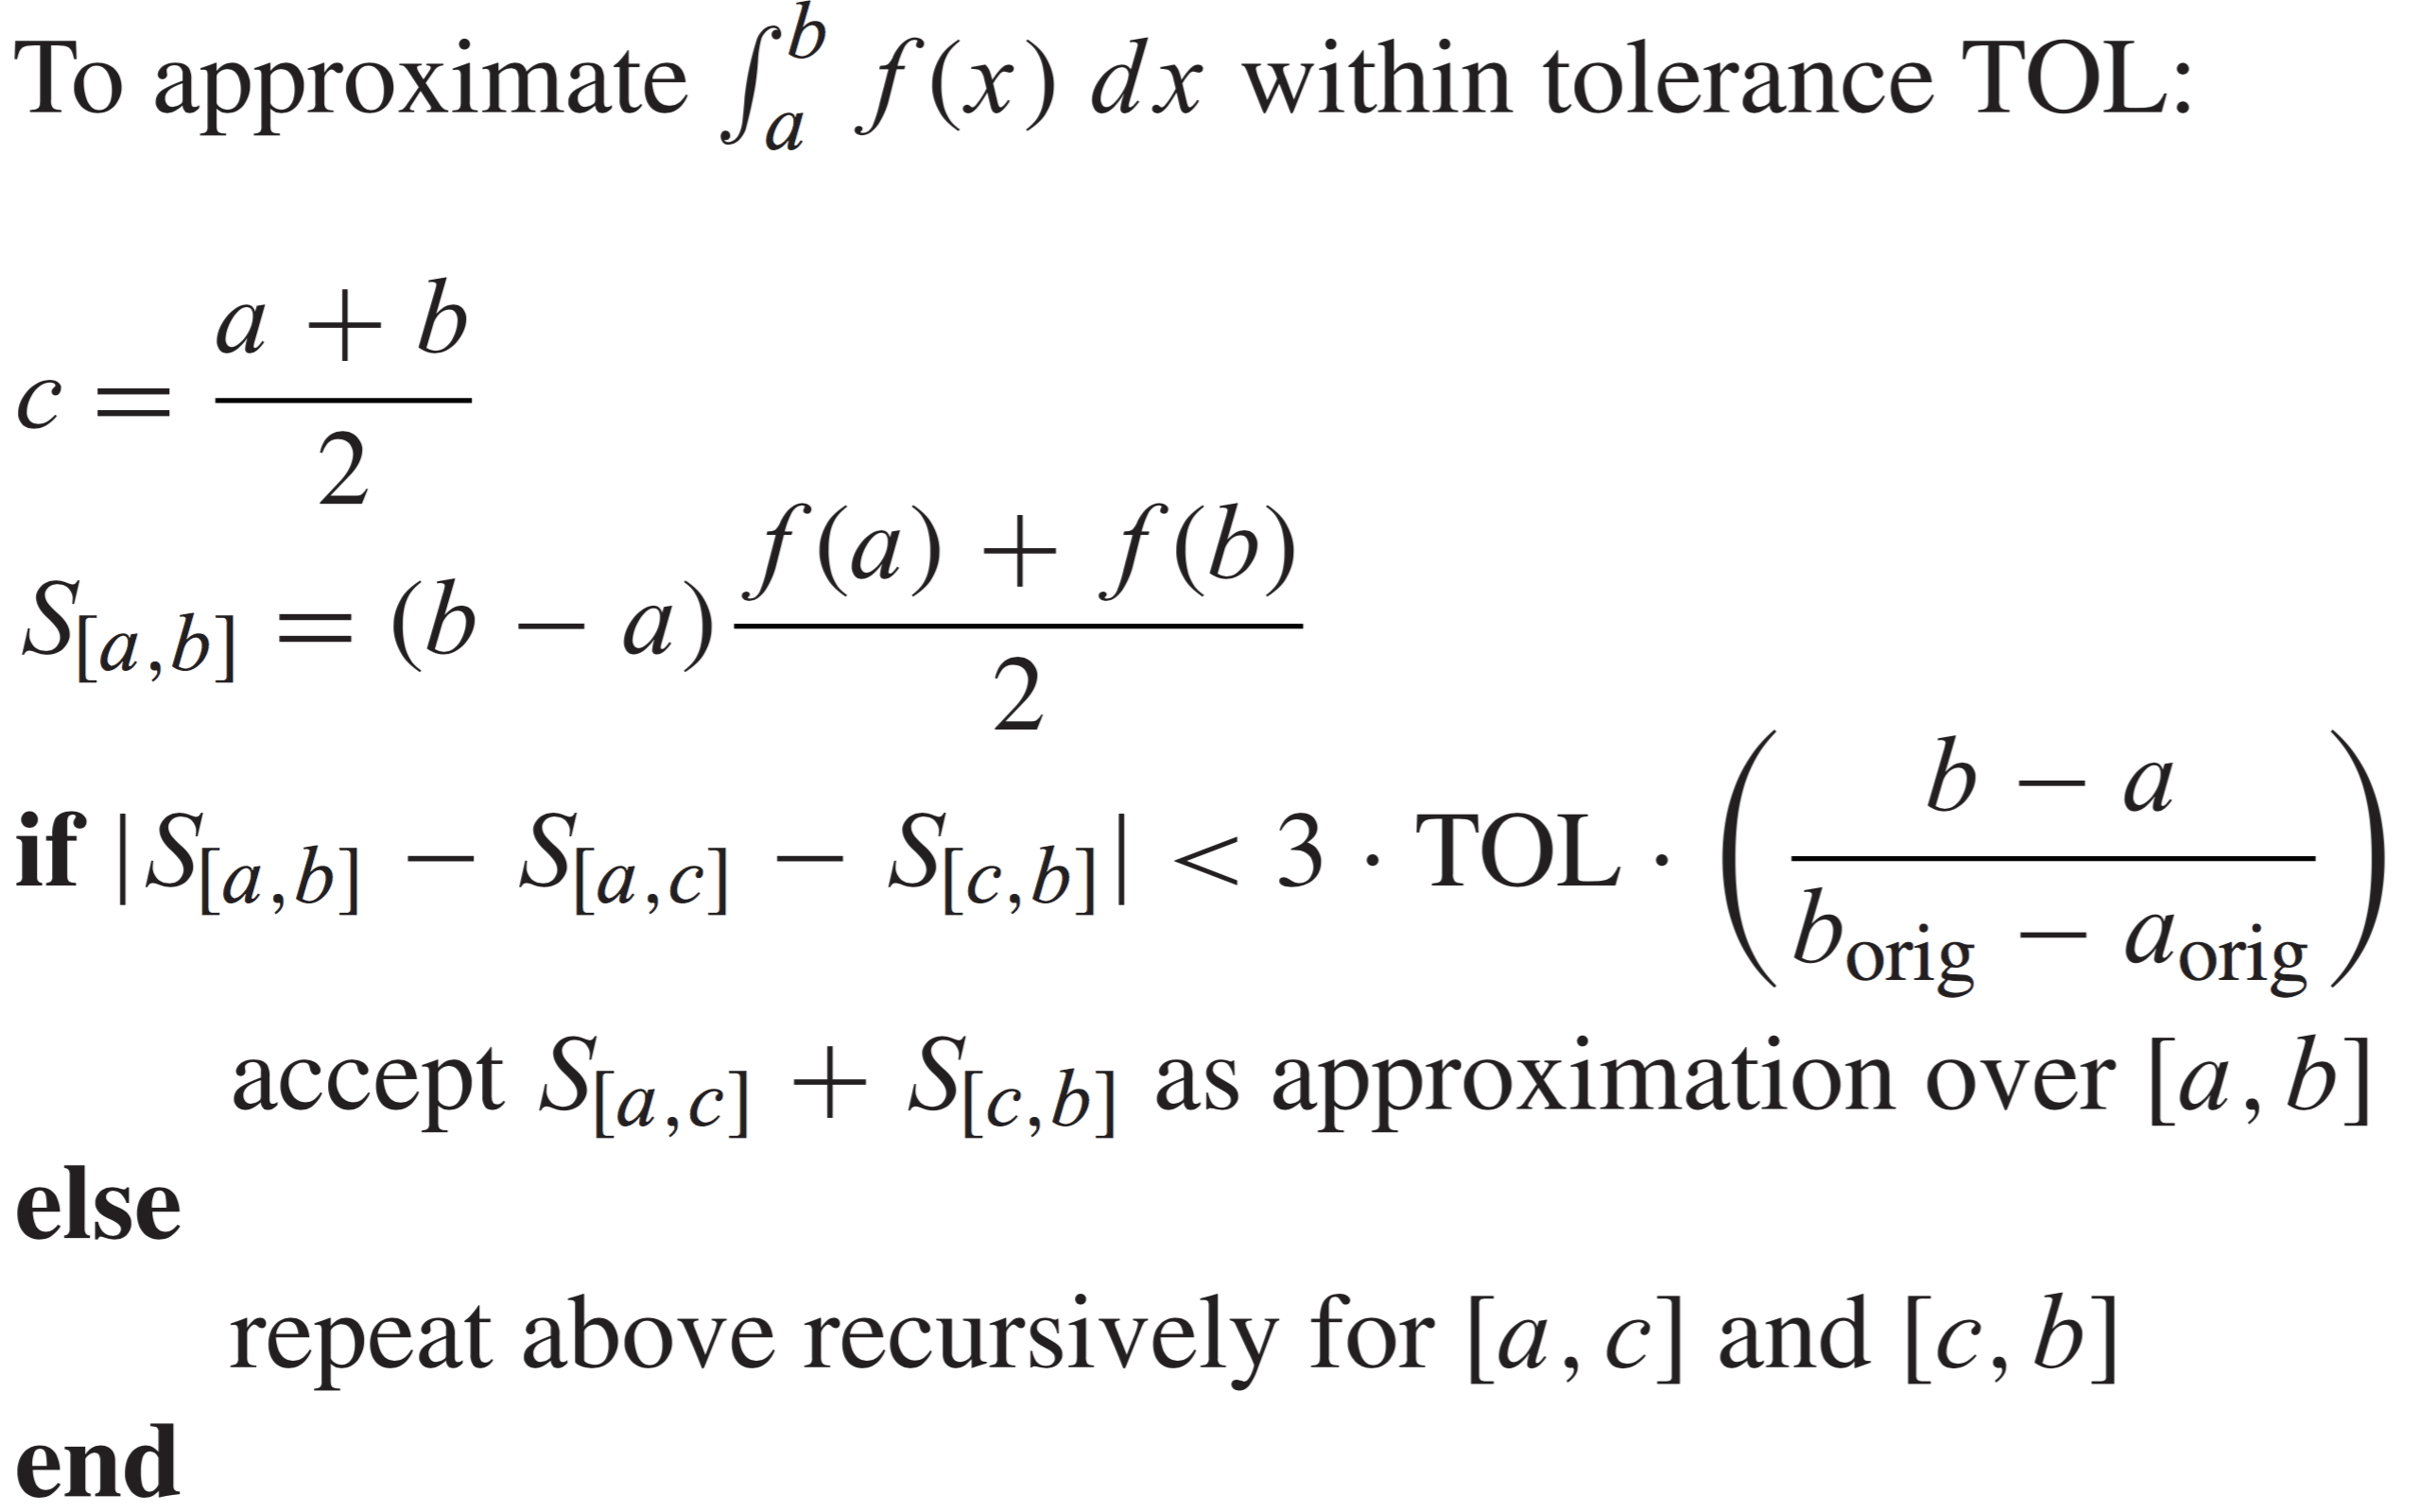
\includegraphics[scale=0.18]{images/adaptive_quadrature.png}
\end{center}

\subsection{Error estimation}
%Do not memorize the exact form of an error estimate for each quadrature, but rather have an idea that they can be derived from either a Taylor series expansion or an interpolation error estimate, when necessary.
Integrate the interpolation error (see "Interpolation Error") or perform a Taylor series expansion and integrate the error term (see "Taylor Method of order $k$"). 
\section{ODEs}
% Should I add Leipshitz definiton?
Solving the initial value problem
$$
\begin{cases}
y' = f(t,y) \\
y(a) = y_a \\
t in [a,b]
\end{cases}
$$
with...
\subsubsection{Euler's method}
% At the very least, backward/forward Euler.
\begin{align*}
w_0 = & y_0 \\
w_{i+1} = & w_{i} + h f(t_i, w_i)
\end{align*}

\subsubsection{Backwards Euler Method}
Use when the diff. equation is \textbf{stiff}, i.e. attracting solutions are surrounded with fast-changing nearby solutions, the linear part of $y$ on the r.h.s.is large and negative.
\begin{align*}
w_0 = &y_0 \\
w_{i+1} = & w_{i} + h f(t_i, w_{i+1})
\end{align*}
Solving this implicit equation for $w_{i+1}$ might require the use of Newton's method.
 
\subsubsection{Explicit Trapezoid Method}
%Trapezoid method can also be easily stated if you remember the trapezoid quadrature/explicit Euler. 
\begin{align*}
w_0 &= y_0 \\
w_{i+1} &= w_i h \frac{h}{2}(f(t_i,w_i)) + f(t_i + h, w_i + hf(t_i,w_i)))
\end{align*}

\subsubsection{Local and global error}
%Concepts of local/global errors and how local truncation error can be derived for a given method using a Taylor series expansion. 
\begin{definition}
A function $f(t,y)$ is \textbf{Lipschitz continuous} in the variable $y$ on the rectangle $S = [a,b] \times [\alpha, \beta]$ if there exists a constant $L$ (called the \textbf{Lipschitz constant}) satisfying
$$
\abs{f(t,y_1) - f(t,y_2)} \leq L\abs{y_1 - y_2}
$$
for each $(t,y_1)$,$(t,y_2)$ in $S$.
\end{definition}

\begin{definition}
The \textbf{global truncation error} is defined as $g_i = \abs{w_i-y_i}$, and the \textbf{local truncation error} is defined as $e_{i+1} = \abs{w_{i+1} - z(t_{i+1})}$. $z$ is the correct solution of the one-step IVT starting at $w_i$.
\end{definition}

\begin{theorem}
If $f(t,y)$ has a Lipschitz constant $L$, and the ODE solver has a local truncation error $e_i \leq C h^{k+1}$, then the solver (which is of order $k$) has a global truncation error
$$
g_i = \abs{w_i - y_i} \leq \frac{Ch^k}{L}(e^{L(t_i - a)} - 1)
$$
\end{theorem}

\subsubsection{Taylor Method of order $k$}
\begin{align*}
    w_0 & = y_0 \\
    w_{i+1} & = w_i + h f(t_i, w_i) + \frac{h^2}{2} + ... + \frac{h^k}{k!}f^{(k-1)}(t_i, w_i),
\end{align*}
with a respective error term 
$$
y_{i+1} - w_{i+1}  =  \frac{h^{k+1}}{(k+1)!}y^{(k+11)}(c) = \mathcal{O}(h^{k+1}),
$$
where $c \in [t, t+h]$.

%TODO: Should I add definition of Leipschitz and theorem 6.4 about global error?
\subsubsection{Adaptive methods}
%Idea of adaptive methods in general and Runge-Kutta in particular.
Compare $e_i$ or $e_i/max(\abs{w_i}, \theta)$ with the error tolerance, and change $h_i$ as needed. If $e_i \approx ch_i^{p+1}$, the relative tolerance TOL is satisfied when $\text{TOL} \leq ch^{p+1} / \abs{w_i}$. Solving for $h$ gives the new step size
$$
h_{i+1} = 0.8\left(\frac{\text{TOL}\abs{w_i}}{e_i}\right)^{\frac{1}{p+1}} h_i,
$$
with a safety factor of $0.8$.

The error in going from $t_i$ to $t_{i+1}$ can be estimated as $e_{i+1} \approx \abs{z_{i+1} - w_{i+1}}$, where $z$ is a higher order estimate. This is often done with an \textbf{embedded Runge-Kutta pair} that shares much of the needed computations. An example is the order 2/order 3 embedded pair:

\begin{align*}
w_{i+1} = & w_i + h \frac{s_1 +s_2}{2} \\
z_{i+1} = & w_i + h \frac{s_1 + 4s_3 + s_2}{6}
\end{align*}

where

\begin{align*}
    s_1 = & f(t_i,w_i) \\
    s_2 = & f(t_i + h,w_i + hs_1) \\
    s_3 = & f(t_i + \frac{h}{2},w_i + \frac{h}{2}\frac{s_1 + s_2}{2})
\end{align*}

with an error estimation of

$$
e_{i+1} \approx \abs{w_{i+1} - z_{i+1}} = \abs{h\frac{s_1 - 2s_3 + s_2}{3}}.
$$

You should still use $z_{i+1}$ to advance the step (\textbf{local extrapolation}).
\section{DFT/FFT}
%You should have a pretty good idea about the definition of DFT and be able to apply it, and derive its properties. Of course different definitions use different normalization constants, and the definition used in the book is absolutely symmetric with respect to direct/inverse transforms (I can never remember which one is which), so simply state the definitions of direct/inverse transforms that you are using at the exam! 
\begin{definition}
The \textbf{Discrete Fourier Transform} of $x = [x_0,...,x_{n-1}]^T$ is the $n$-dimensional vector $y = [y_0,...,y_{n-1}]^T$, where $w = e^{-i2\pi/n}$ and
$$
y_k = \frac{1}{\sqrt{n}} \sum_{j=0}^{n-1}x_j w^{jk}.
$$
\end{definition}

Or in matrix terms
\begin{gather*}
\begin{bmatrix}
    y_0 \\
    y_1 \\
    y_2 \\
    \vdots \\
    y_{n-1}
\end{bmatrix}
=
\begin{bmatrix}
    a_0 + ib_0 \\
    a_0 + ib_1 \\
    a_0 + ib_2 \\
    \vdots \\
    a_{n-1} + ib_{n-1}
\end{bmatrix}
=
F_n
\begin{bmatrix}
    x_0 \\
    x_1 \\
    x_2 \\
    \vdots \\
    x_{n-1}
\end{bmatrix},
\end{gather*}

where the \textbf{Fourier matrix}, $F_n$, is equal to
$$
F_n = \frac{1}{\sqrt{n}}
\begin{bmatrix}
    w^0 & w^0 & w^0 & \hdots & w^0 \\
    w^0 & w^1 & w^2 & \hdots & w^{n-1} \\
    w^0 & w^2 & w^4 & \hdots & w^{2(n-1)} \\
    w^0 & w^3 & w^6 & \hdots & w^{3(n-1)} \\
    \vdots & \vdots & \vdots & \ddots & \vdots \\
    w^0 & w^{n-1} & w^{2(n-1)} & \hdots & w^{(n-1)^2}
\end{bmatrix}
$$
The \textbf{inverse Discrete Fourier Transform} is then given by $x = F_n^{-1}y$ or 
$$
x_k = \frac{1}{\sqrt{n}} \sum_{j=0}^{n-1}y_j w^{-jk}.
$$

\subsection{Useful properties of the DFT}
\begin{itemize}
    \item The inverse of the Fourier matrix is the matrix consisting of the complex conjugates of the entries of $F_n$: $F_n^{-1} = \conj{F}_n$.
    \item The Fourier matrix is \textbf{unitary}, that is $\conj{F}_n^T F_n = I$.
    \item The magnitude of a complex vector is: $\magn{\vec{v}} = \sqrt{\conj{\vec{v}}^T \vec{v}}$.
    \item There is no change in magnitude after a unitary matrix multiplication: $\magn{Fv}^2 = \conj{v}^T\conj{F}^T F v = \conj{v}^T v = \magn{v}^2$.
    \item If $\vec{x}$ is real, then $y_0$ is real, and $y_{n-k} = \conj{y_k}$.
    \item $\vec{x_1} \cdot \vec{x_2} = \vec{x_2}^T \vec{x_1}$ and $[F_n \vec{x}]^T = \vec{x}^TF_n^{-1}$.
\end{itemize}

\subsection{The Fast Fourier Transform}
%Idea about FFT and its complexity. 
The FFT uses the following property in order to split DFT$(N)$ into two DFT$(N/2)$s plus $2N-1$ extra operations

\begin{gather*}
 \sum_{n=0}^{N-1}x_n e^{-2 \pi i n k / N} \\
= \sum_{n=0}^{N/2-1} x_{2n}e^{-2 \pi i(2n)k/N} + \sum_{n=0}^{N/2-1} x_{2n+1}e^{-2 \pi i(2n+1)k/N} \\
= \sum_{n=0}^{N/2-1} x_n^{\text{even}}e^{-2 \pi i n k /(N/2)} + e^{-2 \pi i k / N} \sum_{n=0}^{N/2-1} x_n^{\text{odd}}e^{-2 \pi i n k /(N/2)}
\end{gather*}

\subsection{Trigonometric interpolation}
%Connection between Fourier transform, trigonometric interpolation, ...
Given the interval $[c,d]$ and positive integer $n$, let $t_j = c + j(d-c)/n$ for $j = 0,...,n-1$, and let $\vect{x}=(x_0,...,x_{n-1})$ denote a vector of $n$ numbers. Define $\vec{a} + \vec{b}i = F_n \vec{x}$. Then the complex function
$$
Q(t) = \frac{1}{\sqrt{n}} \sum_{k=0}^{n-1} (a_k + i b_k) e^{i 2\pi k (t-c)/(d-c)}
$$
satisfies $Q(t_j) = x_j$ for $j= 0,...,n-1$. Furthermore, if the $x_j$ are real, the function
\begin{gather*}
P(t) = \frac{1}{\sqrt{n}} \sum_{k=0}^{n-1} \left( a_k \cos{\frac{2 \pi k (t-c)}{d-c}} - b_k \sin{\frac{2 \pi k (t-c)}{d-c}} \right)
\end{gather*}
satisfies $P(t_j) = x_j$ for $j = 0, ... ,n-1$, assuming $n$ is even. Using the cosine and sine addition formulas together with the fact that $y_{n-k} = \conj{y_k}$, $P(t)$ can be simplified to

\begin{gather*}
    P_n(t) = \frac{a_0}{\sqrt{n}}  
    + \frac{2}{\sqrt{n}} \sum_{k=1}^{n/2-1} \left( a_k \cos{\frac{2 \pi k (t-c)}{d-c}} - b_k \sin{\frac{2 \pi k (t-c)}{d-c}} \right) \\
    + \frac{a_{n/2}}{\sqrt{n}} \cos{\frac{n \pi (t-c)}{d-c}}
\end{gather*}

\subsection{Fourier filtering/compression relevant to the project}
%... and a general idea about filtering/compression (~ at the level of the project).
\begin{itemize}
    \item \mcode{MATLAB} uses a non-unitary normalization for its Fourier transformation, such that $F_n x$ is computed by \mcode{fft(x)/sqrt(n)}, and $F_n^{-1} y$ by \mcode{ifft(y)*sqrt(n)}.
    \item Given $n$ data points, the best least squares trigonometric function with $m < n$ terms can be found by interpolating with $n$ terms, and then only keep the first $m$ terms (dropping the higher frequencies, called a \textbf{low pass filter}).
    \item A \textbf{high pass filter} can be made by dropping the lower frequency components.
\end{itemize}

\end{multicols*}

\end{document}
